\chapter{Project Research}
This section investigates similar projects and products. Market analysis was conducted in the fall of 2018 to create an overview of the market. 70+ key figures from the Danish and international music business - musicians, recording producers, touring personnel, etc. - were interviewed for an investigation of their consumption patterns, gear run downs, their requests for useful features and the pitfalls of their gear. \newline

The most experienced users are the so-called \textit{backline technicians} (or backliners) that travel/tour with a touring artist or band to set up, tear down and maintain the artists' instruments and gear. In addition to setting up and tearing down the gear, the backline technician often operates electronics that run parts of the show such as backing tracks on some chosen device, MIDI changes, tune guitars/basses during the perfomance - In general to assist in making the artist's performance to run smoothly without unnecessay interruptions. \newline

The most experienced backliners actively explore and research new technologies and products in between tours and/or during their spare time. Some even modify hardware and software to suit their clients' needs. And some backliners - usually on tours with larger production budgets - even design customized systems. \newline

Indeed, touring personnel - whether they are backliners, sound engineers, lighting engineers, etc. - are passionate about their job and they continually explore solutions to make a performance to run even more smoothly. \newline

The common denominator in the interviews is the critical need for stability. Some of the technologies outlined later in this section have trade-offs: Some sacrifice user-friendly GUIs to ensure stability, some trade-offs are loss in audio quality to ensure stability and user-friendly GUI and vise versa. \newline

As several of the available technologies heavily rely on laptops and home-made systems during performances, the incentive to produce Showman is to remove laptops from the perfomance scenario to avoid hiccups during a show. \newline

Following subsections briefly introduce the most popular tehcnoloqies used currently by touring artists and their personnel with a list of their pros and cons. This chapter concludes with an introduction of Showman's desired features. \\

\section{Similar Projects}
This subsection investigates similar projects from Scandinavia. \\

\subsection{Interactive Performance System}
Mircea Gabriel Eftemie, Medialogy-alumni from Aalborg University developed a system called '\textbf{Interactive Performance System}', a visual system for concert performances: https://videnskab.dk/kultur-samfund/heavy-metal-pa-universitetet. The project was developed using Open Source technology as his Bachelor's Project with fellow students Thomas Wisbech, Lasse Wingreen and Brenly Bernard. \newline

The purpose of the system was to display theatrical and visual elements during performance without the aid of technical personnel to enhance the performance experience for the audience. The system combined two inputs: A static and dynamic input. The static inputs were prepared beforehand. The static inputs were controlled by an input during the performance partly from a webcam that filmed the audience and the artists and partly from a microphone that recorded and transmitted the audio on stage. \newline

Mircea played guitar in now-defunct Mnemic that utilized the Interactive Performance System. The project was put to rest after Mnemic's dissolution and the project status remains unclear. \\

\subsection{The Dark Player}
Members of Swedish band Darkane developed a system for backing track playback device called '\textbf{The Dark Player}' after expressing dissatifaction with current products available. I am in the process of tracking down the members to investigate their system further. \\

\section{Similar Products}
Digital Audio Workstations are the hub for 99 percent of all modern musicians and producers. (Source: https://ask.audio/articles/the-top-11-most-popular-daws-you-voted-for) \newline

Products similar to Showman exist in many forms: From simple iPods to complex systems, artists can pick and choose any system available in several configurations depending on financial status. However, some proves to be too unreliant, unstable or reliant on other pieces of hardware to function as intended. The subsubsections below outlines the most widely used products. This subsection conludes with Showman's intended features. \\

\subsection{Cymatic Audio LP-16}
The LP-16 (http://cymaticaudio.com/lp-16-productpage/) is a multi-track player for live perfomances that spares the user of using laptop and computer audio interface in a live environment. Its primary use is backing tracks, but its other features include virtual sound checks, triggering synthesizers or samplers, drigin light shows and controlling devices. \\

\begin{figure}[H]
\centering
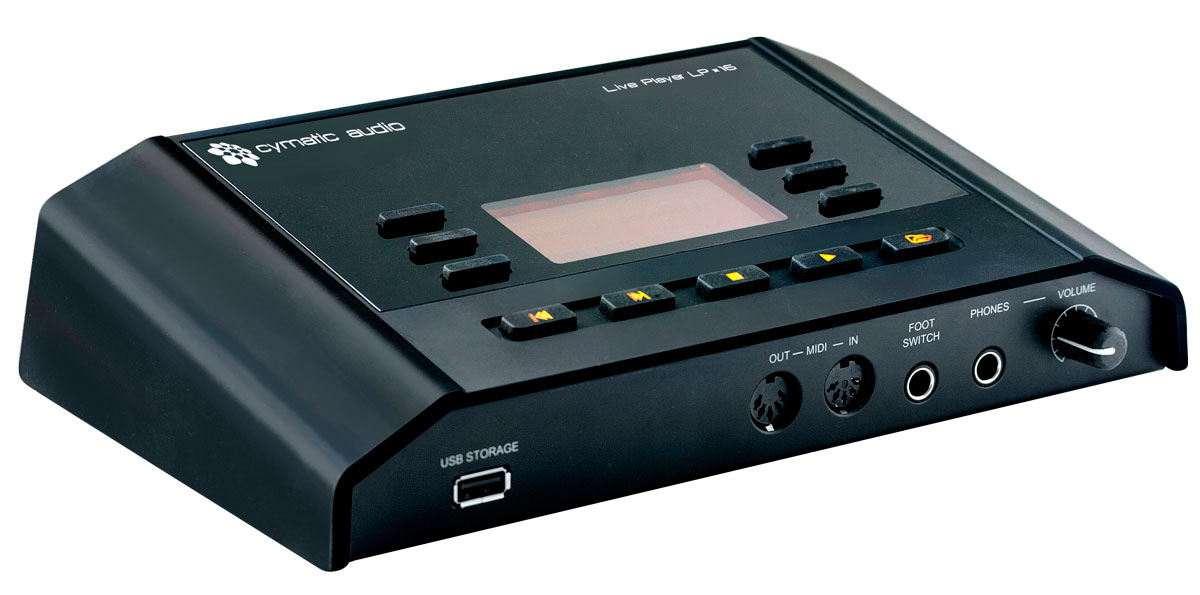
\includegraphics[scale=0.2]{./pictures/lp.png}
\caption{Press photo of Live Player LP-16. Source: http://cymaticaudio.com/lp-16-productpage/}
\label{fig:lp.png}
\end{figure}

\begin{itemize}
\item Direct from USB hard drive multi-track playback: 16 tracks at 24-bit, 44.1/48 kHz
\item Creation and editing of setting and playlist offline with software uTool
\item 16 \textit{unbalanced} analog 1/4'' tip-sleeve outputs
\item Mac OS-X and Windows PC compatible
\item 249 EUR at thomann.de
\end{itemize}

\begin{figure}[H]
\centering
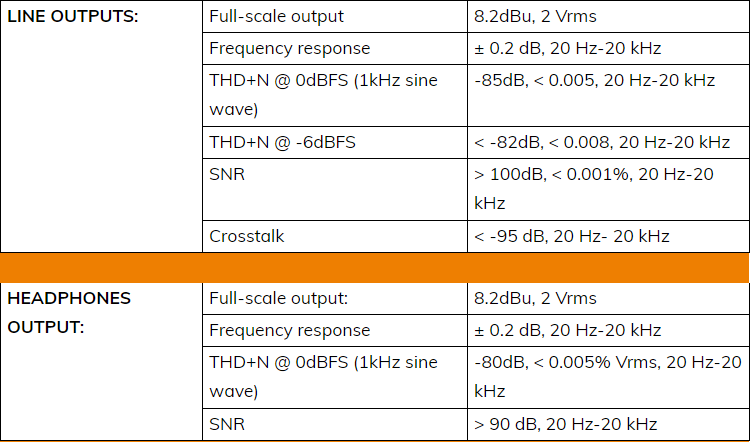
\includegraphics[scale=0.7]{./pictures/lp16.png}
\caption{Selected specifications of Cymatic Audio LP-16 Live Player}
\label{fig:lp16.png}
\end{figure}

Minimum requirements for connection to mixing board: \\

\begin{itemize}
\item Up 16 x 1/4'' tip-sleeve jack-cables: 14.90 EUR for the sssnake MPP8030 at thomann.de
\item Up to 16 x line drivers: 2 x 103 EUR (Behringer DI800 Ultra-DI PRo v2 from thomann.de): 206 EUR
\item USB hard drive: SanDisk USB 2.0 Stick Cruzer: 19.95 EUR
\item Assuming local venue provides XLR-cables: Minimum expenses to use LP-16: 489.85 EUR
\end{itemize}

Using low-budget and low-quality accessories, the LP-16 is still relatively expensive considering memory is external USB hard drive, making it vulnerable to vibrations on stage.

\subsection{Ableton Live}
Ableton Live is an audio MIDI sequencer and digital audio workstation (DAW) software for Mac OS-X and Windows PC, purchased with proprietary license. Ableton Live is designed to be an instrument for live performances as well as a tool for composing, recording, arranging, mixing, and mastering. \newline

Ableton Live need an audio interface for connection to mixing board. Applications are wide and very much individual - Users purchase audio interface to suit their work flow and requirements.  Prices for Ableton Live start at 209 euros for a Student license.\\

Minimum requirements for connection to mixing board: \\
\begin{itemize}
\item Ableton Live software installed on chosen laptop (Mac OS-X or Windows PC) \\
\item Audio interface (they start from 2 channel outputs and upwards) \\
\end{itemize}

\begin{figure}[H]
\centering
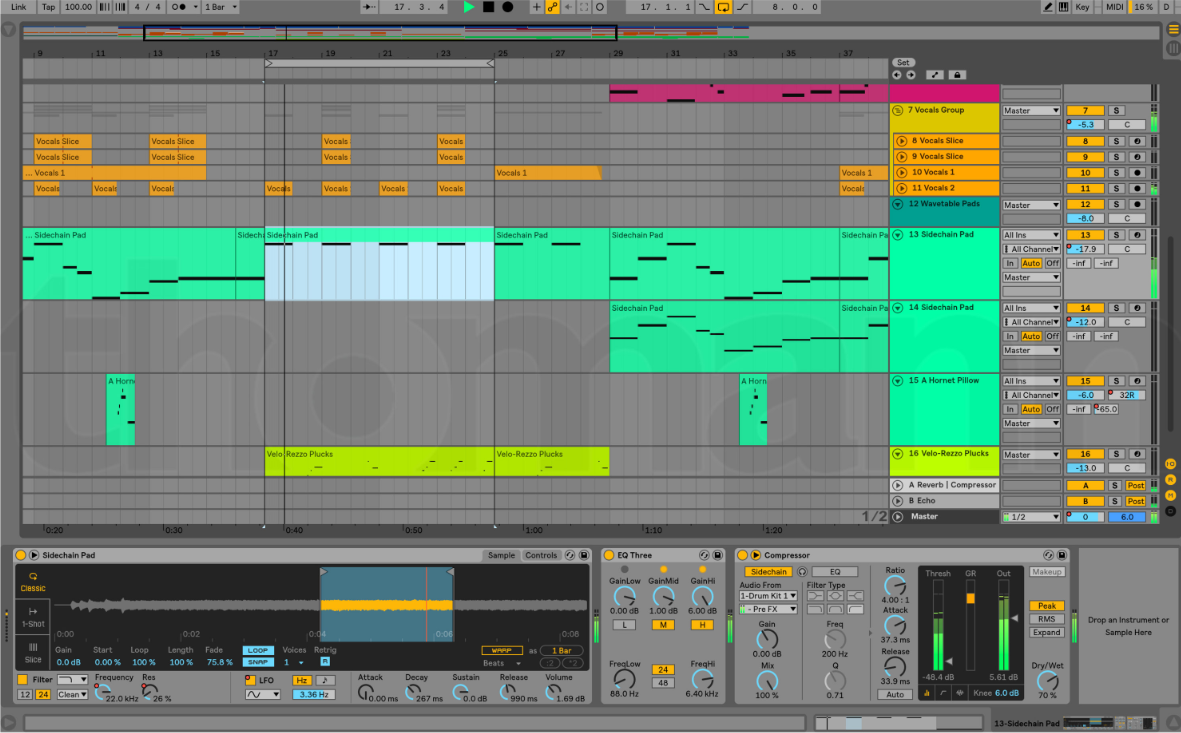
\includegraphics[scale=0.4]{./pictures/ableton.png}
\caption{Screenshot of Ableton Live GUI environment. Source: https://www.thomann.de/dk/ableton\_live\_10\_intro.htm}
\label{fig:ableton.png}
\end{figure}

\subsection{QLab}
QLab is a free download that combines audio, video and lightning control in one package (http://figure53.com/qlab/). QLab controls playback of these element during a live perfomance. The operator triggers events such as light-, audio- and video-cue(s) in a cue list, which contain cues to trigger an event that the user edited. \newline

\textbf{Audio Playback:} QLab allows end-user or designer to align audio files in sequential order. Once inserted in cue list, end-user can manipulate by looping, change amplitude, volume, fades, etc. End-user need external audio interface to route the audio to mixing board. More on audio interface later. \\

\textbf{Video Playback:} End-user or designer can add video to cue list for synchronization and modification in real time. End-user need video card to route video to a screen. Speed of CPU and video card can affect quality of video playback. Does not support Windows PC - Mac OS-X only. \\

\textbf{Pricing:} QLab cost from 4.00 USD/day for a 24-hour license to 999.00 USD for a one-time license purchase with all the features. Free version has limited features.

\begin{figure}[H]
\centering
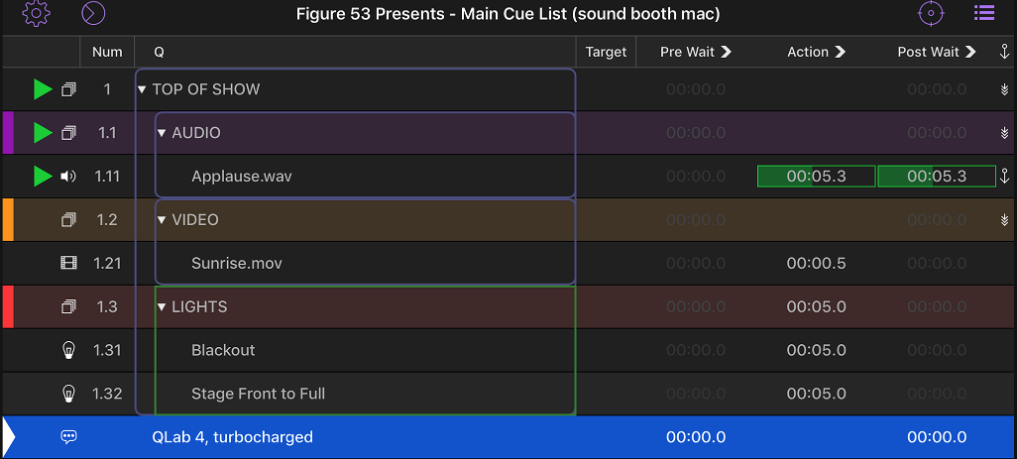
\includegraphics[scale=0.8]{./pictures/qlab.png}
\caption{Screenshot of QLab GUI environment. Source: (https://figure53.com/qlab/remote/)}
\label{fig:qlab.png}
\end{figure}

\subsection{Logic Pro X}
Logic Pro X is a DAW and MIDI sequencer software application for the Mac OS-X platform. Logic's primary function is music production, but is also widely used for playback in live performances. \newline

Developed by Apple Inc., the current proprietary license is released macOS. Logic version 5.5.1 wasthe last version bo be released for Windows. Version 6 and onward, Logic is only available for Mac OS. Like QLab, Logic need external audio interface to connect with mixing board. \\
 
\begin{figure}[H]
\centering
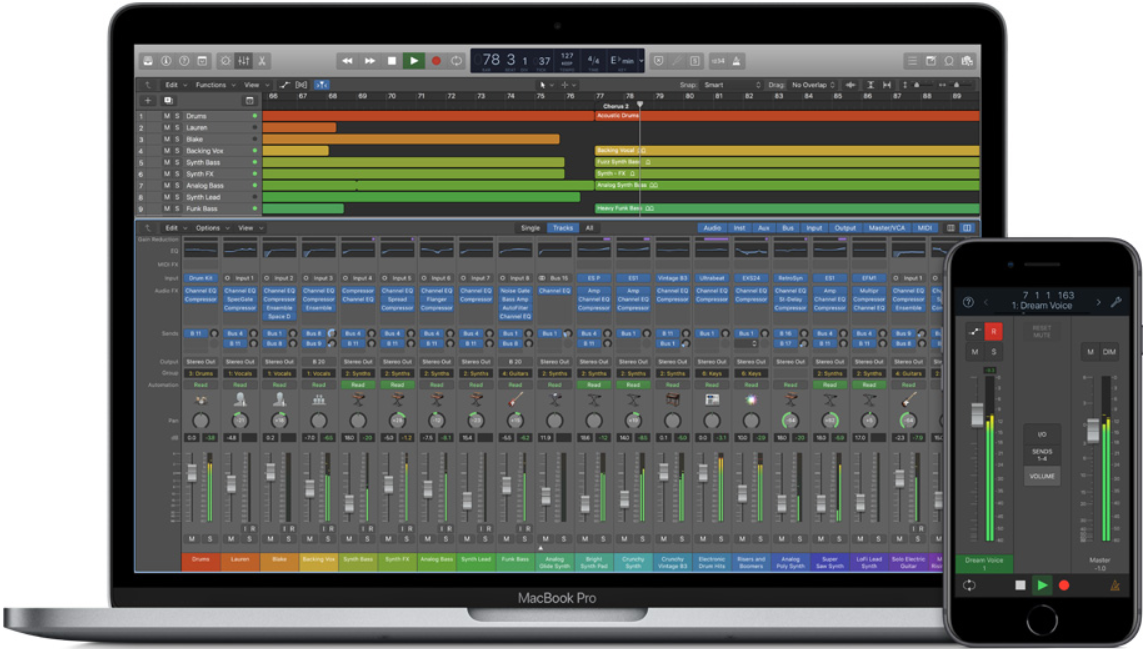
\includegraphics[scale=0.4]{./pictures/logic.png}
\caption{Screenshot of Logic software application. Source: https://www.apple.com/logic-pro/resources/}
\label{fig:logic.png}
\end{figure}

\textbf{Price:} 199.99 USD in App Store. \\

\subsection{MainStage}
Even though Apple's Logic Pro X is capable of playback of multichannel of audio, its primary function is music production: Recording and editing of audio tracks. \newline

MainStage is designed exclusively for live performances with a few key features, play back of pre-recorded backing tracks being the most notable feature. Like QLab and Logic, MainStage need external audio interface to connect with mixing board. \\
 
\begin{figure}[H]
\centering
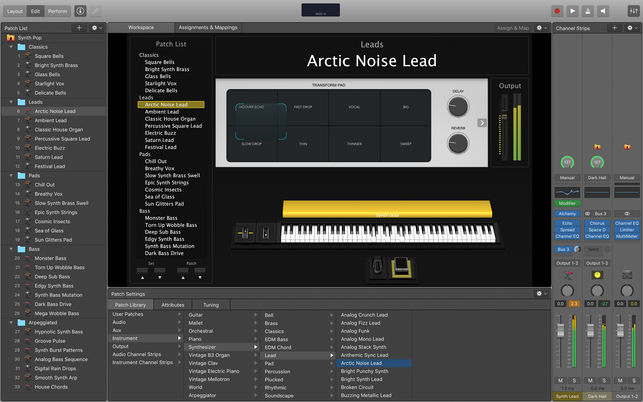
\includegraphics[scale=0.4]{./pictures/mainstage.png}
\caption{Screenshot of MainStage software application. Source: https://itunes.apple.com/dk/app/mainstage-3/}
\label{fig:mainstage.png}
\end{figure}

\textbf{Price:} 29.99 USD in App Store. \\

\subsection{Pro Tools}
Pro Tools is a DAW developed and release by Avid Technologies for Windows and masOS. Its many features include audio recording, music production, editing, post production, etc. \newline

Pro Tools can run as standalone software \textit{or} operate using external A/D converters, PCIe cards with onboard DSPs. Like QLab, Logic and MainStage, Pro Tools need external audio interface to connect with mixing board. \\

\begin{figure}[H]
\centering
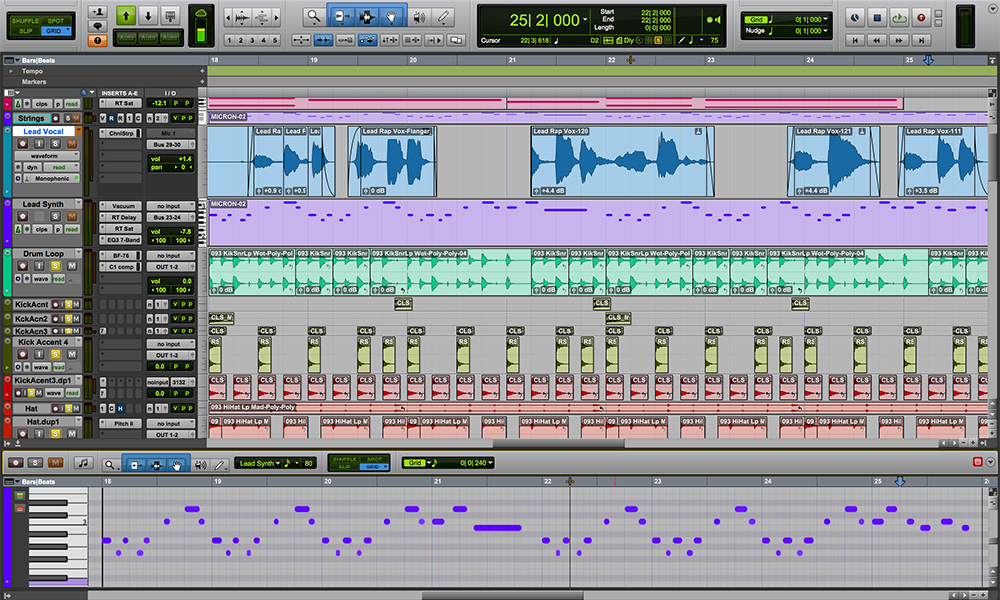
\includegraphics[scale=0.3]{./pictures/protools.png}
\caption{Screenshot of Pro Tools software application. Source: https://www.avid.com/pro-tools/features/}
\label{fig:protools.png}
\end{figure}

\textbf{Price:} From free software for Pro Tools | First with limited features to  559,00 EUR for one-time purchase with annual upgrade plan.

\subsection{Open Source Products}
Quite a few Do-It-Yourself (DIY) builders, enthusiasts, hobbyists and likeminded individuals have attempted to produce similar products with various degrees of success. \newline

Several open source technologies are available for product development:\textbf{Arduino} (https://www.arduino.cc/), \textbf{Raspberry Pi} (https://www.raspberrypi.org/) and \textbf{BeagleBone Black} (https://beagleboard.org/black) counts as the most widely used technologies. \newline

As Showman is intended for market release for consumers and prosumers, open source solutions are not within the scope of the project at the moment as additional research in open source regulations and their marketability is necessary - A research that can lead the project to a sidetrack and the time frame does not allow for in-depth investigations. \\

\subsection{Showman}
The intended features for Showman is shown in Figure ~\ref{fig:showman.png}

\begin{figure}[H]
\centering
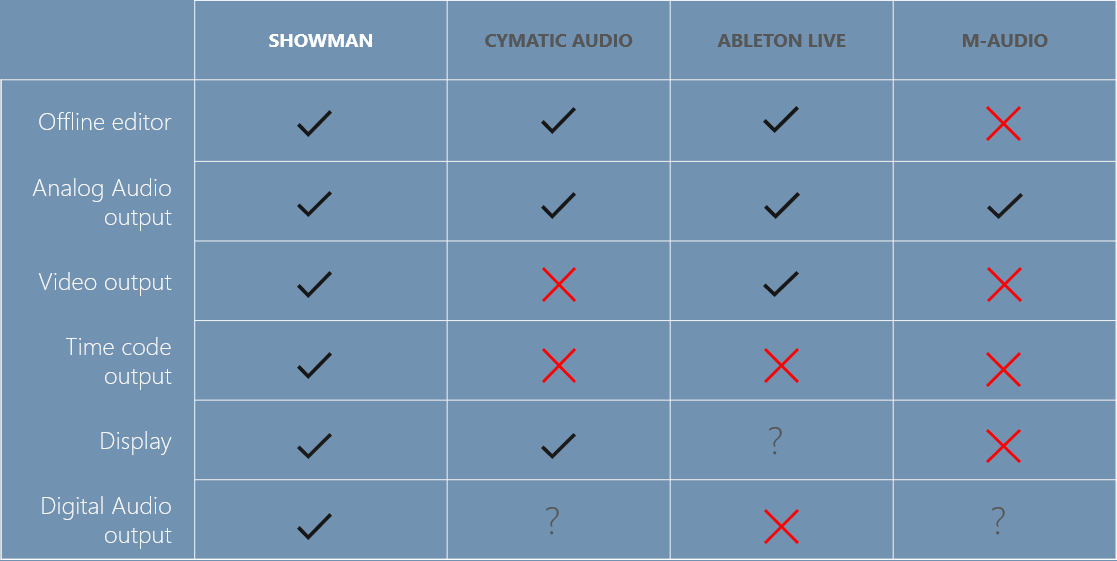
\includegraphics[scale=0.5]{./pictures/showman.png}
\caption{Intended features for Showman with a comparison matrix of competing producers.}
\label{fig:showman.png}
\end{figure}

\section{Literature}
As mentioned in the description, a research in these subjects are needed for design, implementation and test of Showman: \\

For design and implementation of the device, a research is needed in: \\

\begin{itemize}
\item Circuit/hardware design
\item D/A audio converters
\item Standardized audio input/output formats
\item Audio file formats
\item Standardized video input/output formats
\item Video file formats
\item Time codes for synchronizatio
\item User feedback for feasible GUI design
\end{itemize}

Selected chapters from: \\
\textbf{Ken C. Pohlmann}: Principles of Digital Audio Sixth Edition. (\textbf{ISBN: 987-0-07-166346-5}). This is the starting point for the literature. Additional textbooks from the AU Library or from other sources will be investigated when additional information becomes relevant. \\

\textbf{Eddy Bøgh Brixen}: Praktisk Elektroakustik 3. udgave. \textbf{ISBN: 9788791117206}. This textbook introduces several audio concepts necessary for Showman's features such as XLR-plugs, file formats, etc. \\ 

\textbf{User Manuals}: User manuals from competing producers are necesary to understand the design process. Some of these contain block diagrams that can be useful for Showman when modified to suit Showman's needs. \\

\textbf{Datasheets}: In addition to textbooks, datasheets for relevant parts will be investigated thoroughly and evaluated upon before implementation. \\

\textbf{GUI Design}: Research in GUI design is a must have for design of software application GUI. It was the project's wish to work as a team with a more experienced programmer and student from the \textbf{Information and Communication Technology} branch of ASE, but none were available. However, 2 external programmers has expressed interest in occassional assistance and guidance during design and implementation process of GUI.